\section{Методы моделирования супрануклеосомной структуры хроматина}
% сделать на основе https://docs.google.com/document/d/1A_RRCcKiU5YPzdSMHhqiwX-g2PkqbeQ4iB5KrB0_MFI/edit?usp=sharing

    В последние годы благодаря совершенствованию экспериментальных технологий наметилась долгожданная конвергенция методов структурной биологии и методов геномики в изучении организации хроматина на молекулярном уровне. Благодаря успехам крио-электронной микроскопии, мы получаем все больше информации о структуре не только нуклеосом, но и супрануклеосомных структур, а благодаря развитию методов геномики и 3-D геномики все более высокого разрешения, стало возможным определять контакты между локусами ДНК с суб-нуклеосомным разрешением (в частности, методы Micro-C, Micro-C-XL и др.) и определять положение и состав нуклеосом вдоль генома (напр. методы MNase-seq, MNase-ChIP-seq). Возникает необходимость в интерпретации экспериментальных данных и построении физических молекулярных моделей укладки хроматина на супрануклеосомном уровне с учетом реальных геометрических и топологических параметров молекул белков и ДНК, а также динамического характера этих взаимодействий.

    Так как изучение организации хроматина на супрануклеосомном уровне довольно давно представляет собой фундаментальную задачу для молекулярной и клеточной биологии (примем за дату начала год открытия нуклеосомы и структуры в виде ``бусин на нити'' - 1974 \cite{kornberg_chromatin_1974}), было разработано множество подходов к молекулярному моделированию укладки нуклеофиламента. Большую часть прошедшего времени сомнений в концепции 30-нанометровой фибриллы не возникало (идею 30-нанометровой фибриллы предложили в 1980 году, серьезные аргументы против появились в 2000-ых, 2010-ых  см., например, \cite{joti_chromosomes_2012,razin_chromatin_2014}). Поэтому подавляющее число работ по молекулярному моделированию хроматина на супрануклеосомном уровне являются по сути работами по моделированию 30-нанометровой фибриллы, что, не умаляя их методологической значимости, значительно снижает ценность результатов и приводит к необходимости проведения работ по молекулярному моделированию хроматина на супрануклеосомном уровне с учетом современных знаний о нем.  При этом изучение предыдущей литературы по данной теме все-таки необходимо, так как ее авторы достигли значительных результатов в разработке математического и концептуального  аппарата для моделирования хроматина на этом уровне вообще. Например, в работе 2015 года Norouzi, D. \& Zhurkin, V. B. Topological Polymorphism of the Two-Start Chromatin Fiber \cite{norouzi_topological_2015} авторы с помощью своей модели изучили все возможности организации двухстартовой хроматиновой фибриллы (есть два гипотетических типа организации 30-нанометровой хроматиновой фибриллы: соленоидная - одностартовая фибрилла - и зигзагом - двухстартовая фибрилла - причем тип фибриллы коррелирует с длиной ликерного участка), т.е. смоделировали все возможные ее конформационные варианты. Фибриллы моделировали симметричными и регулярными, а для расчетов вводилось 4 параметра суперспирализации: кручение, подъем, наклон нуклеосом и диаметр. Энергия фибриллы задавалась как сумма четырех слагаемых: эластической энергии линкерной ДНК, стерического отталкивания, электростатики (рассчитываемой с помощью кулоновского потенциала), феноменологического взаимодействия между двумя ``сложенными в стопку'' нуклеосомами. При оптимизации энергии фибриллы с учетом параметров суперспирализации исследователи впервые обнаружили два типа топологического перехода в ней: путем резкого на 360 градусов поворота в кручении линкера и путем скрещивания линкеров. Даже при моделировании структуры, отличной от 30-нанометровой фибриллы, эти принципы могут быть релевантными, так как позволяют рассчитать такие общие вещи, как энергию комплекса ДНК-нуклеосома, его оптимальную геометрию в зависимости от длины линкеров и внешних факторов. Эти же авторы  в более поздней  работе того же года продолжали исследовать топологический полиморфизм хроматиновой фибриллы, пытаясь установить связь между длиной линкеров и спецификой сверхспирализации ДНК (связанной с уровнем транскрипции). Интересно, что для нахождения оптимальной конформации линкерной ДНК использовался мезоскопический подход: ДНК моделируется динуклеотидными ``шагами'', его траектория описывается с помощью шести параметров: Tilt, Roll, Twist, Shift, Slide, Rise. Мезоскопический подход был  предложен в статье Olson et al., 1993 \cite{olson_influence_1993}, данные шестимерные координаты - в работе Dickerson et al., 1989 \cite{dickerson_definitions_1989}. Оба этих концептуальных инструмента широко используются в моделировании хроматина на низких уровнях компактизации (10-нанометровой фибриллы и следующем) и никак не зависят от концепции 30-нанометровой фибриллы, что делает их полезными и для моделирования альтернативных этой фибрилле структур. Крайне эффективным для молекулярного моделирования супрануклеосомного уровня компактизации хроматина являются методы, основанные на принципах Монте-Карло. Познакомиться с ними можно, например, в работе — Norouzi, D. \& Zhurkin, V. B. Dynamics of Chromatin Fibers: Comparison of Monte Carlo Simulations with Force Spectroscopy \cite{norouzi_dynamics_2018}. Шаги симуляции следующие: случайный выбор одной пары оснований в подвижном линкере и изменение его шести параметров, обновление позиций нуклеосом в нуклеосомном массиве, вычисление разницы в энергии между старым и новым состоянием и выполнение теста Метрополиса. Варьируя величину внешних сил, степень развернутости (unwrapping) нуклеосом, длину нуклеосомных повторов (NRL - nucleosome repeat length) - среднее расстояние между центрами соседних нуклеосом и значение энергии стэкинга (stacking energy), исследователи провели серию симуляций, каждая из которых включала около 100 миллионов описанных выше шагов. Подобный подход, особенно его вариант - моделирование путем имитации отжига - позволяет довольно эффективно находить глобальный энергетический минимум в заданной системе.
    
    Также часто применяется для решения задач моделирования хроматина на разных уровнях организации метод огрубленного моделирования (coarse-grained). Суть метода состоит в представлении молекул и молекулярных структур (например, нуклеосом) простыми телами и поверхностями: сферами, цилиндрами, плоскостями. Такое приближение значительно упрощает вычисления и позволяет проводить однозначный анализ за приемлемое время. Однако при этом исходные данные подвергаются соответствующей деформации - результат моделирования соответствует им не полностью, он также зависит от выбранной стратегии огрубления. Хроматиновые фибриллы и их динамику обычно моделируют как цепочки из шаров или как червеобразные структуры \cite{korolev_systematic_2018,savelyev_molecular_2009,ozer_chromatin_2015}. Несмотря на популярность метода огрубленного моделирования в области изучения структуры хроматина, он является далеко не оптимальным для решения этих задач: исходные данные не используются полностью, искажаются, что может быть критичным, когда речь заходит об изучении укладки 10-нанометровой фибриллы, так как образуемая ею структура зависит от не учитываемых в огрубленных методах параметров - например, длины линкера \cite{norouzi_topological_2015,nikitina_dna_2017,norouzi_topological_2015}. Для адекватного моделирования структуры хроматина требуется основывать его на данных высокого разрешения (например, современных протоколов Hi-C), причем они не должны искажаться так сильно, как в методе огрубленного моделирования. Таким образом необходимо разработать новый, более чувствительный к данным и параметрам наподобие длины линкеров подход. 

    Важно отметить, что большинство описываемых выше подходов основаны на ``закрытом'' программном обеспечении. Авторы либо не предоставляют доступа к программному обеспечению, либо оно является слабо используемым, поскольку к нему нет описания, либо возникают проблемы с переносимостью.

\begin{figure} [h!]
    \centering
    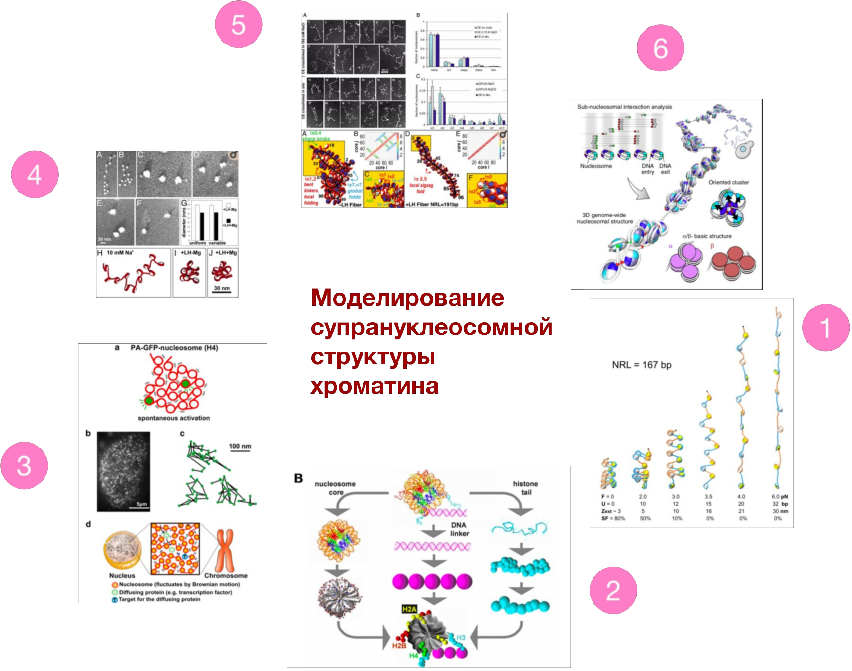
\includegraphics [width=\textwidth]{images/p1/part1_4_cm/part1_4_cm_f6.pdf}
    \caption[Подходы к моделированию супрануклеосомной структуры]{Подходы к моделированию супрануклеосомной структуры, в том числе с учетом экспериментальных данных. (1) - Молекулярная динамика с использованием принципов Монте-Карло \cite{norouzi_dynamics_2018}; (2) - Огрубленное моделирование \cite{schlick_monte_2009}; (3) - (6) : интегративные методы. (3) - Моделирование на основе данных метода Single nucleosome imaging  - отображения одиночных нуклеосом \cite{maeshima_chromatin_2014}; (4), (5) - Моделирование на основе данных метода EMANIC - метода обнаружения нуклеосом с помощью электронной микроскопии \cite{grigoryev_evidence_2009}, \cite{grigoryev_hierarchical_2016}); (6) - Моделирование супрануклеосомной структуры на основе данных модифицированного Micro-C   \cite{ohno_sub-nucleosomal_2019}}.
    \label{fig:p1_4:f6}
\end{figure}


    Важным подходом является интеграции различных экспериментальных данных при построении моделей - данный подход называется интегративным моделированием. В применении к супрануклеосомной структуре он на наш взгляд развит весьма слабо. На данный момент по данным литературы известна лишь одна попытка интеграции данных Micro-C с методами моделирования. Работа опубликована в 2019 году \cite{ohno_sub-nucleosomal_2019}. В ней приведены довольно убедительные доказательства существования определенных супрануклеосомных структур в геноме пекарских дрожжей, альтернативных отвергнутой  хроматиновой фибрилле, - хроматиновых альфа-тетраэдров и бета-ромбов - то есть этой работой был сделан большой шаг на пути к определению структуры хроматина на до сих пор не исследованных уровнях компактизации генома. Молекулярное моделирование проводилось на основании теоретической модели нуклеосомы - как комплекса из гистонового октамера и ассоциированной с ним ДНК — и данных Micro-C, позволяющих различать точки ``входа'' и ``выхода'' ДНК в/из нуклеосом. Такой комбинированный метод был назван Hi-Co. Само моделирование проводилось с помощью подхода имитации отжига в методе молекулярной динамики. Имитация отжига была необходима для оптимизации позиций и ориентаций отдельных нуклеосом, остальные структурные факторы, такие как, например,  линкерная ДНК (ее длина), были неявно включены в потенциалы и по сути не рассматривались детально. Несмотря на важное значение, подходы моделирования в работе Ohno et al.  не вполне реалистичны, так как, например,  отсутствуют в явном виде линкерная ДНК, а следовательно не учитывается влияние топологии и кручения ДНК важные для понимания многих функциональных процессов и состояний в хроматине. Также в подходе авторов не предполагался учет нуклеосом различного типа и возможного откручивания ДНК от нуклеосомы с изменением углов входа/выхода ДНК. Кроме того работа Ohno et al. была посвящена изучению генома дрожжей — это значит, что непосредственной значимостью для медицины она не обладает. Требуется провести аналогичное исследование генома высших, многоклеточных эукариот и человека.

%картинка
\begin{figure} [h!]
    \centering
    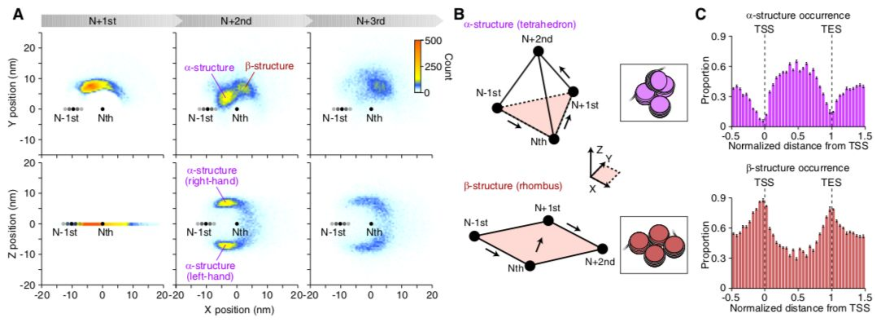
\includegraphics[width=\textwidth]{images/p1/part1_4_cm/part1_4_cm_f7.pdf}
    \caption[Визуализация анализа данные Micro-C, Ohno et al., 2019]{Визуализация результатов анализа взаимного расположения нуклеосом в пространстве и выявленные в результате него мотивы супрануклеосомной структуры ДНК из статьи Ohno et. al, 2019}
    \label{fig:p1_4:f7}
\end{figure}

Для моделирования супрануклеосомной укладки фибрилл алгоритмы, предложенные нами в пункте \ref{sec:p1:int_algo}, могут быть адаптированы путем включения дополнительных данных из экспериментов Micro-C, а также данных о позициях нуклеосом из экспериментов MNase-seq, ATAC-seq (см. Рис. \ref{fig:p1_4:f8}). 
     Расчет обобщенных переменных из атомистической структуры и восстановление координат из набора переменных, описывающих геометрию ДНК в динуклеотидном приближении, производится при помощи программы 3DNA \cite{lu_3dna_2003}, либо при помощи разрабатываемой программной библиотеки PyNAMod.      Учет положения и геометрии белковых компонент можно производить в том же приближении: для этого необходимо определять их ориентацию относительно ключевых динуклеотидов. Например, при определении гистонового ядра нуклеосомы, отсчитывать его положение относительно диадного динуклеотида.
    Дополнительно в физическую модель нуклеосомной фибриллы вводятся парные потенциалы для учета исключенного объема и электростатических взаимодействий между соседними нуклеосомами, что необходимо для учета изменяющих заряд посттрансляционных модификаций гистоновых хвостов.
     При моделировании цепочек нуклеосом, вводятся ограничения на расстояния, описывающие межнуклеосомные контакты. Возможно также введение дополнительного потенциала, позволяющего нуклеосомам смещаться относительно их изначальных положений (что обосновано точностью определения их положения в эксперименте).   В рамках описываемой физической модели нуклеосомной фибриллы можно создавать модели организации хроматина путем применения численных методов минимизации значений функции, например метода градиентного спуска, однако, для обнаружения глобального минимума, а также создания множественной выборки из конфигурационного пространства более применимы стохастические подходы, такие как метод  Монте-Карло с алгоритмом Метрополиса.

\begin{figure} [h!]
    \centering
    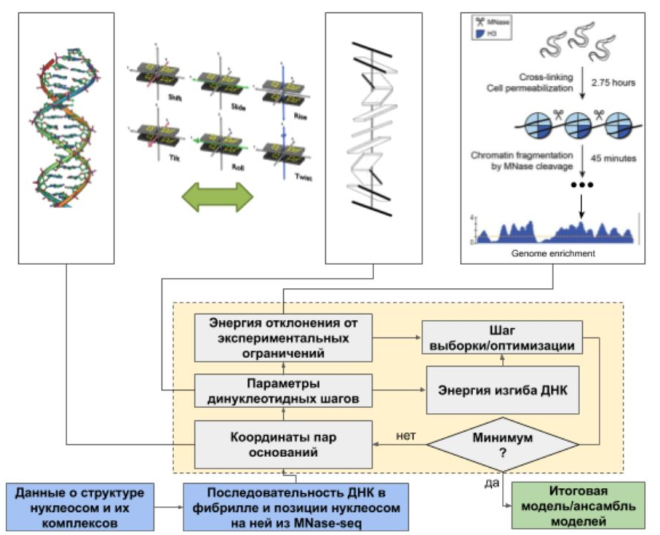
\includegraphics [width=\textwidth]{images/p1/part1_4_cm/part1_4_cm_f8.pdf}
    \caption[Алгоритмы интегративного моделирования нуклеосомных фибрилл]{Алгоритмы интегративного моделирования нуклеосомных фибрилл. Слева вверху - схематическое описание ДНК в приближении динуклеотидных шагов. Справа вверху - сокращенное схематическое представление методов Micro-C/MNase-seq/MNase-ChIP-seq. Снизу - Описание подхода интеграции экспериментальных данных в физическую модель нуклеосомных фибрилл.}
    \label{fig:p1_4:f8}
\end{figure}










